\documentclass{article}
\usepackage{amsmath,amssymb,setspace,verbatim,graphicx,enumerate,enumitem}
\usepackage[top=1in,bottom=1in,left=1in,right=1in,nohead,nofoot]{geometry}
\usepackage{caption}
% \usepackage{subcaption}
% \usepackage{subfig}
% \usepackage{subfloat}
% \usepackage{tabularx}
\usepackage{mdframed}

\newenvironment{Rcode}% environment name 
{%begin code
    \begin{mdframed}
    \#R code
    \begin{small}
}
{%end code
    \end{small}
    \end{mdframed}
}

\newenvironment{console}% environment name 
{%begin code
    \begin{mdframed}
    \#Console
    \begin{small}
}
{%end code
    \end{small}
    \end{mdframed}
}

% \parindent 0in
% \parskip .2in
% \pagestyle{empty} \singlespacing
% %\newcommand{\vect}[1]{\mbox{\boldmath $ #1$}}
% \newcommand{\bv}[1]{\mathbf{#1}}
% \setlist{noitemsep,topsep=0pt,parsep=0pt,partopsep=0pt}


\begin{document}
\title{FDA Homework 1}
\author{Seokjun Choi}
\date{September 30, 2019}
\maketitle

\section{Chapter 1}
\subsection{Problem 1}

The pinch is a dataset included in the fda package. It consists of 151 measurements of pinch force for 20 replications (curves). 

\subsubsection*{(a)  Convert the pinch data to functional objects using 15 B-splines of order four (cubic splines) and plot the 20 smoothed curves on one graph.}
To get the result we want, call the fda package and execute the code below.

\begin{Rcode}
    \begin{verbatim}
b_spline_basis<-create.bspline.basis(c(1,151), nbasis=15)
pinch.F<-Data2fd(1:151, pinch, b_spline_basis)
plot(pinch.F)
    \end{verbatim}
\end{Rcode}
Then we get the result.
\begin{figure}[hh]
    \centering
    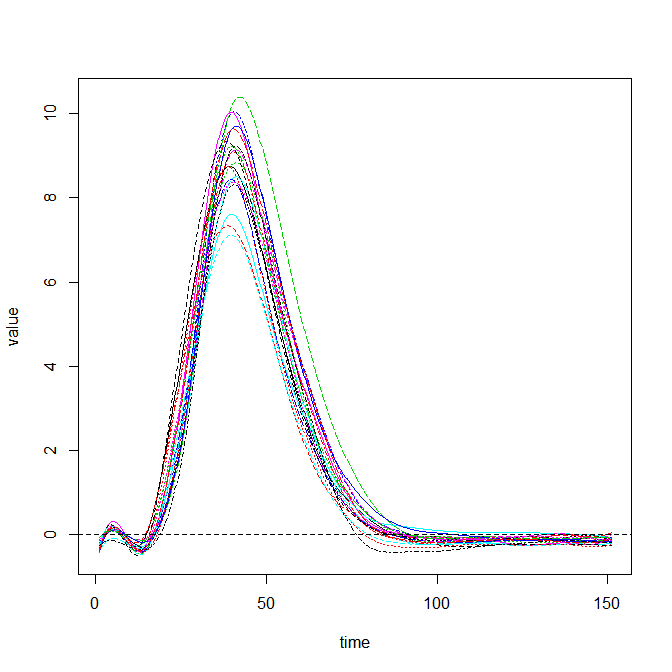
\includegraphics[height=8cm]{pinch_F_plot.png}
    \caption{fitting pinch data using 15 b-splines}
\end{figure}

\newpage
\subsubsection*{(b) Calculate the pointwise mean and SD and add them to the plot.}
For calculation, run the code below.
\begin{Rcode}
    \begin{verbatim}
pinch.F.mean <- mean(pinch.F)
pinch.F.mean$coefs

pinch.F.std <- std.fd(pinch.F)
pinch.F.std$coefs

par(mar=c(4,4,1,1))
plot(pinch.F, col="grey")
plot(pinch.F.mean,lwd=4,add=TRUE)
plot(pinch.F.std, lwd=4, add=TRUE, col="red")
    \end{verbatim}
\end{Rcode}

For analytic expression of pointwise mean and point sd, denote $b_i$ as i-th b-spline of order 4
on domain $[0,120] \subset \Re$. Then
\[Mean(x)=\sum_{i=1}^{16}c_ib_i(x)\]
\[Sd(x)=\sum_{i=1}^{16}s_ib_i(x)\]
where $c_i$ : -0.31109576, 0.73142704, -1.63349675, 2.72475346, 10.93667264, 6.03218354, 2.28791198, 0.34957598, -0.09607592, -0.16637125, -0.11240041, -0.15664938, -0.10293668, -0.16311715, -0.11897440
and $s_i$ : 0.0846463, 0.1182031, -0.0996403, 0.9735739, 0.6517423, 1.1140145, 0.5002106, 0.3255844, 0.1166337, 0.1232983, 0.0639047, 0.0869009, 0.0824064 0.0776430, 0.07207136
respectively. 

And here is a plot of the result.
\begin{figure}[hh]
    \centering
    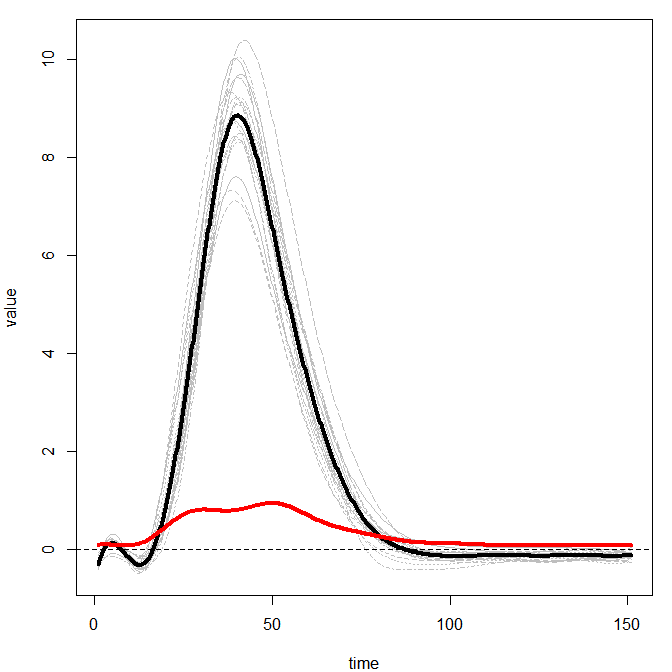
\includegraphics[height=8cm]{pinch_F_mean_var_plot.png}
    \caption{fitting pinch data using 15 b-splines: \\ Mean is black bold curve, and Sd is red bold curve.}
\end{figure}


\newpage
\subsubsection*{(c) Graph the perspective and contour plots of the sample covariance function $\hat{c}(t,s)$ of the pinch curves.}

We can easily do them by using for var.fd function of fda package and persp, contour function of R.
\begin{Rcode}
    \begin{verbatim}
pinch.F.cov <- var.fd(pinch.F)
dim(pinch.F.cov$coef) #15*15
grid <- 1:15
pinch.F.cov.mat = eval.bifd(grid, grid, pinch.F.cov)
par(mfrow=c(1,2), mar=c(4,4,1,1))
persp(grid, grid, pinch.F.cov.mat, xlab="s", ylab="t", zlab="cov(s,t)")
contour(grid, grid, pinch.F.cov.mat)
    \end{verbatim}
\end{Rcode}

Result plots are here.

\begin{figure}[hh]
    \centering
    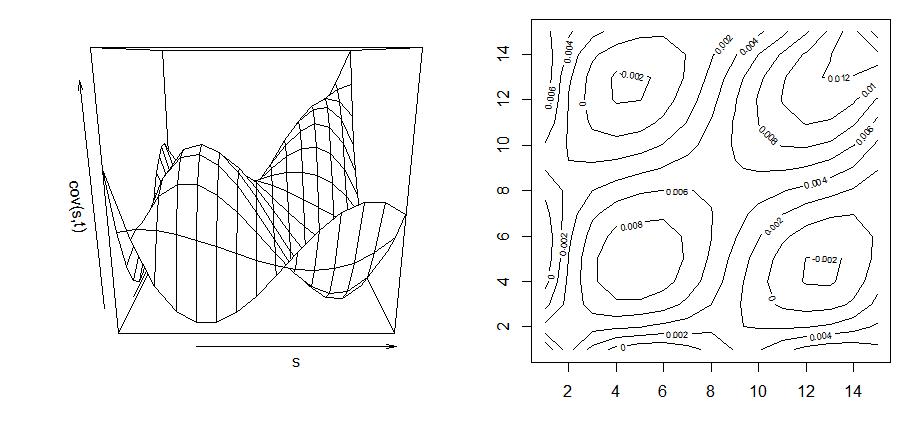
\includegraphics[height=8cm]{pinch_F_cov_persp_contour_plot.png}
    \caption{fitting pinch data using 15 b-splines: \\ covariance perspective plot and contour plot.}
\end{figure}

\newpage
\subsubsection*{(d) Graph the first four EFPC’s of the pinch data. How many components do you need to explain 90\% of variation?}

Let's do PCA with 4 components following the instruction of problem, and see the proportions of variance of each component for determining number of components for 90\% explanation.

\begin{Rcode}
    \begin{verbatim}
par(mfrow=c(1,1))
pinch.F.pca = pca.fd(pinch.F, nharm=4)
plot(pinch.F.pca$harmonics, lwd=3)
pinch.F.pca$varprop
    \end{verbatim}
\end{Rcode}

Firstly, Plot the first 4 eigenfunctions.

\begin{figure}[hh]
    \centering
    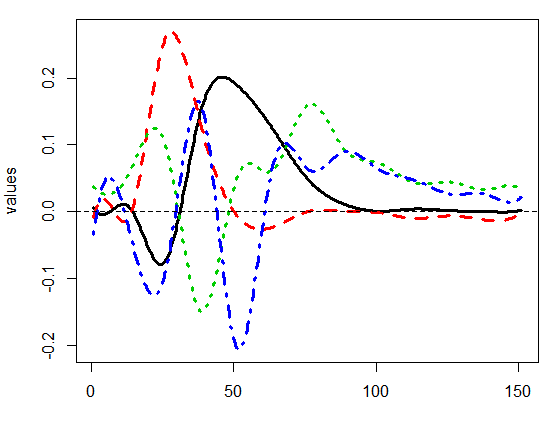
\includegraphics[height=8cm]{pinch_F_pca_4components_plot.png}
    \caption{fitting pinch data using 15 b-splines and do PCA: \\ first 4 components.}
\end{figure}

And the ouput of last line is

\begin{console}
    \begin{verbatim}
> pinch.F.pca$varprop
[1] 0.67225632 0.24845297 0.04603548 0.01933904
    \end{verbatim}
\end{console}

Since the sum of first 2 proportion is 0.9207093, we need only 2 components to reach 90\% level of explanation of variation.


\newpage
\subsection{Problem 2}

For this problem, download the R package fds and use the data set of the United States Federal Reserve interest rates, FedYieldcurve,
which contains the monthly interest rates from January 1982 to June 2009.
The x-values are the maturity terms of 3, 6, 12, 60, 84 and 120 months which can be identified with the $t_j$ in this chapter.
The y-values are the interest rate of the United States Treasury obligations due in x months which can be identified with the $x_n(t_j)$,
where n is a month in the range January 1982 to June 2009.


Firstly Note that, in R code, variable names are set by
\begin{Rcode}
    \begin{verbatim}
yield = FedYieldcurve
terms = yield$x
    \end{verbatim}
\end{Rcode}
FedYieldcurve is in fds package.

\subsubsection*{(a) On one graph, plot the interest rates $x(t_j)$ for January 1982 and for June 2009 against the maturity terms $t_j$. How do the interest rates in these two months compare?}
Run the code below and get a plot before discuss about comparing yield rates.
\begin{Rcode}
    \begin{verbatim}
plot(terms, yield$y[,1], pch=15, ylab="Yield", ylim=c(0,16)) 
points(terms, yield$y[,330], pch=16)
    \end{verbatim}
\end{Rcode}
\begin{figure}[hh]
    \centering
    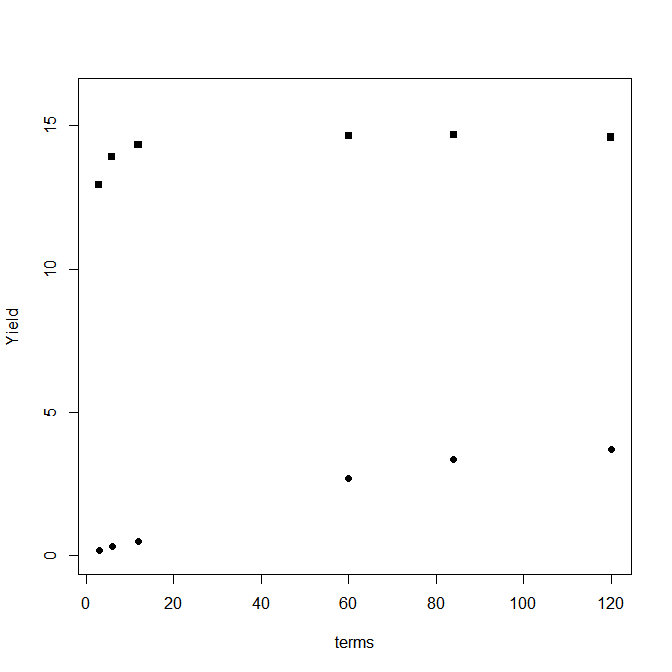
\includegraphics[height=8cm]{yield_2terms.png}
    \caption{yield points of Jan 1982 and June 2009}
\end{figure}
At the maturity of the data exist, we can compare yield rate directly by calculating absolute value of difference.
But for other maturity value, we should use more than data themself. We may use interpolation technique, or other fitting method like LSE or time series analysis's,
but here are FDA class, so use method of FDA's! :)

\newpage
\subsubsection*{(b) Convert the yield data to functional objects using bspline basis with four basis functions. 
Calculate and plot the the mean yield function. What is the average behavior of interest rates as a function of the maturity?}

Execute the code below for following the first and second directions of problem.
\begin{Rcode}
    \begin{verbatim}
b_spline_basis = create.bspline.basis(c(1,120), nbasis=4)
yield.F = Data2fd(terms, yield$y, b_spline_basis)
plot(yield.F, col='gray')

yield.F.mean = mean(yield.F)
plot(yield.F.mean,lwd=4,add=TRUE)
    \end{verbatim}
\end{Rcode}
The result plot is,
\begin{figure}[hh]
    \centering
    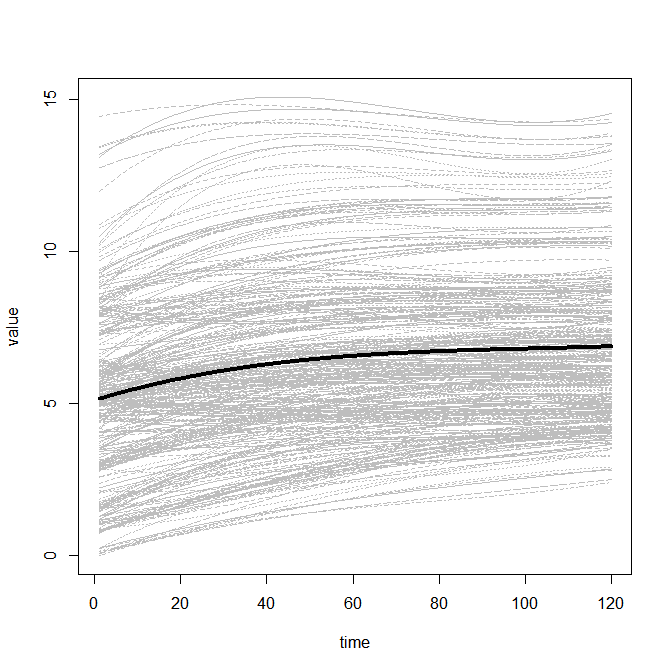
\includegraphics[height=8cm]{yield_bspline4fit}
    \caption{Fitting yield data using b-spline 4 basis:\\Bold curve indicates mean.}
\end{figure}
The mean curve has increasing shape generally, but the slope goes flatter with maturity becoming longer.

\newpage
\subsubsection*{(c) Plot the first principal component of the interest rate curves. What percentage of variance does this component explain? Interpret the plot and the percentage of variance.}
Run the below code to perform PCA with one component.
\begin{Rcode}
    \begin{verbatim}
yield.F.pca = pca.fd(yield.F, nharm=1)
plot(yield.F.pca$harmonics, lwd=3, , ylim=c(-1,1))
yield.F.pca$varprop
    \end{verbatim}
\end{Rcode}

The second line gives the plot of the component function.
\begin{figure}[hh]
    \centering
    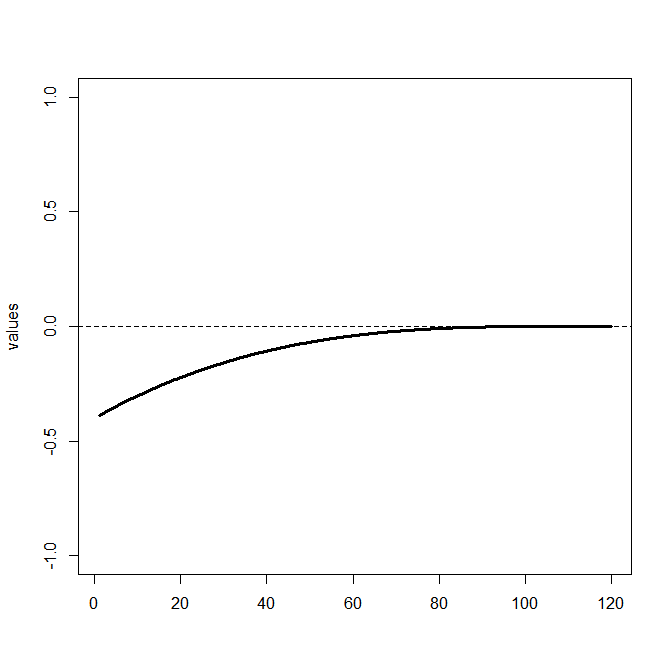
\includegraphics[height=8cm]{yield_bspline4fit_pca_1comp.png}
    \caption{Fitting yield data using b-spline 4 basis:\\ First component of pca.}
\end{figure}

Since overall functions has similar form as we view at Figure 6, the shape of the component is also similar to them, especially mean.

\begin{console}
    \begin{verbatim}
> yield.F.pca$varprop
[1] 0.999982
    \end{verbatim}
\end{console}

Likewise, the proportion of explained variation has high value consisting the above context.

\newpage
\subsection{Problem 6}
In this section we expressed \(x_n(t)=\sum_{m=1}^{M}c_{nm}B_m(t)\). One can show that
\[\bar{x}_N(t)=\sum_{m=1}^{M}a_mB_m(t) \]
and
\[\hat{c}(t,s)=\sum_{m=1}^{M}\sum_{k=1}^Mb_{mk}B_m(t)B_k(s)\]
Find expressions for the coefficients $a_m$ and $b_{mk}$ assuming that the
$B_m(t)$ are an orthonormal basis:
\[\int B_m(t)B_k(t)=1_{m=k}\]
%

Happily, the solution of this problem is in our lecture note, so I repeat the contents.
Firstly for sample mean, observe that
\[\bar{x}_N(t)=\frac{1}{N}\sum_{n=1}^{N}x_n=\frac{1}{N}\sum_{n=1}^{N}\sum_{m=1}^{M}c_{nm}B_m(t)=\sum_{m=1}^{M}(\frac{1}{N}\sum_{n=1}^{N}c_{nm})B_m(t)\]
so if we set \(a_m=\frac{1}{N}\sum_{n=1}^{N}c_{nm}\), we get the expression that we want.
And for sample covariance,
\[\hat{c}(t,s)=\frac{1}{N-1}\sum_{n=1}^{N}(x_n(t)-\bar{x}(t))(x_n(s)-\bar{x}(s))\]
then where \(\tilde{c}_{nm}=c_{nm}-a_m\),
\[=\frac{1}{N-1}\sum_{n=1}^{N}\sum_{m=1}^{M}\sum_{k=1}^{M}\tilde{c}_{nm}\tilde{{c}}_{nk}B_{m}(t)B_{k}(s)\]
\[=\sum_{m=1}^{M}\sum_{k=1}^{M}(\frac{1}{N-1}\sum_{n=1}^{N}\tilde{c}_{nm}\tilde{{c}}_{nk})B_{m}(t)B_{k}(s)\]
so if we set \(b_{mk}=\frac{1}{N-1}\sum_{n=1}^{N}\tilde{c}_{nm}\tilde{{c}}_{nk}\), 
or equivalently using matrix notation \(b_{mk}=(N-1)^{-1}\mathbf{c}^T\mathbf{c}\), we get what we want.



\newpage
\section{Chapter 2}
\subsection{Problem 1}
Verify the equality,
\[\int_{0}^{T}[L(x)(t)]^2dt=\pi\omega^5\sum_{j=2}^{J}j^2(j^2-1)^2(a_j^2+b_j^2)\]
with harmonic acceleration operator \(L(X)(t)=\omega^2x^{(1)}(t)+x^{(3)}(t), \omega=2\pi/T\) \\
and Fourier basis \(x_{J}(t)=c_0+\sum_{j=1}^{J}\{a_j\sin{\omega jt}+b_j\cos{\omega jt}\}\)

For a start, I'll calculate $x^{(i)}(t), i=1,3$. For notational simplicity, I omit subscript J. The results are
\[x^{(1)}(t) = \sum_{j} \{a_j\omega j \cos{\omega jt} - b_j\omega j \sin{\omega jt}\}\]
\[x^{(3)}(t) = \sum_{j} \{-a_j\omega^3 j^3 \cos{\omega jt} + b_j\omega^3 j^3 \sin{\omega jt}\}\]
I notice that when j=1, L become 0 operator. So we can exclude to j=1 case in summation. \\
Then, our operator are actually
\[L(x)(t)=\sum_{j}\{a_j\omega^3(j-j^3)\cos{wjt} + i\frac{1}{i}b_j\omega^3(j^3-j)\sin(wjt)\}\]
Then, using definition of complex sine and cosine function, we can rewrite L as
\[L(x)(t)=\sum_{j}\frac{\sqrt{(a_j+b_j)^2\omega^6j^2(j^2-1)^2}}{2}e^{i\omega jt}\]
Then, by Plancherel's identity,
\[\frac{\omega}{2\pi} \int_{0}^{T}|L(x)(t)|dt = \frac{1}{2}\sum_{j}(a_j+b_j)^2\omega^6j^2(j^2-1)^2\]
Multiplying $\frac{2\pi}{\omega}$ to both term, we get the equation which we want.


\newpage
\subsection{Problem 2}
Proceed with FedYieldcurve data, which contains the monthly Federal Reserve interest rates, cf. Problem 1.6.2.

\subsubsection*{(a) Smooth the interest rates (yields) in January 1982 using a B–spline basis 
with four basis functions. Plot the raw and smoothed interest rates on one graph.}
\subsubsection*{(b) Re-fit the January 1982 yields using a penalized smoothing based on six basis functions 
(as many as data points) with the smoothing parameter $\lambda = 1$, 
and the second derivative as the penalty operator. Add the smooth in red to the graph you obtained 
in part (a) and comment on the result.}
\subsubsection*{(c) Repeat part (b) with several other smoothing parameters $\lambda$. Which $\lambda$ gives the most informative smooth curve?}



\newpage
\subsection{Problem 5}
In this problem, we will explore some potential dangers of curve alignment. 
A bump function centered at a value $c_0$, with radius $r_0$, and amplitude $a_0$ is defined as 
\begin{equation*}
    f(x) = \begin{cases}
        a_0\exp{\{-(1-(\frac{x-c_0}{r_0}^2)^{-1})\}} &\text{if } |x-c_0|<r_0 \\
        0 &\text{otherwise}
    \end{cases}
\end{equation*}
\subsubsection*{(a) Simulate a functional sample over the unit interval each with a sample size of 50 from the Mat\'{e}rn process. 
For the first half of the sample, set the mean function equal to the bump function with parameters $(c_0,r_0,a_0)=(3/8,1/4,5)$.
For the second half use $(c_0,r_0,a_0)=(5/8,1/4,5)$.
You may choose the values for the Mat\'{e}rn covariance function as well as the number of points sampled per curve.
Plot all of the curves and include a curve for the overall mean function.}
\subsection*{(b) Align the curves using continuous registration. Plot the resulting curves and include a mean function. Comment on any differences with (a) and if the registered curves exhibit any odd patterns.}
\subsection*{(c) Carry out an FPCA with one PC on the unaligned and aligned curves separately. 
For each, do a simple linear regression of the score onto a dummy variable (coded 0/1) 
indicating which type of mean the function had (i.e. is it from the first or second half of the sample). 
Calculate a p-value to determine if the estimated slope parameters you get are significant. 
Compare with the aligned and unaligned curves. What did aligning do to the p-value? 
You may want to rerun your simulations a few times to see how the p-values change.}
\subsection*{(d) Come up with one potential setting/application 
where you might lose something if you align. Make up whatever scenario you like, but think it through.}

\end{document}